\newcommand\UniversiteAdi{Niğde Ömer Halisdemir Üniversitesi}
\newcommand\BolumAdi{MEKATRONİK BÖLÜMÜ}
\newcommand\DersKodu{MKT2002}
\newcommand\DersAdi{BİLGİSAYARLI KONTROL SİSTEMLERİ}
\newcommand\SinavAdi{Ödev 4}
\newcommand\SinavTarihi{10.03.2025}
\newcommand\SinavSaati{10:00}
\newcommand\SinavSuresi{90dk}

\pagestyle{fancy}
\fancyhf{} % clear existing header/footer entries
\fancyhead[R]{Öğrenci No:\hspace{4.5cm}}
\fancyhead[L]{Ad Soyad:\hspace{7cm}}
\noindent
\begin{tabular}{
    p{0.15\linewidth}
    p{0.15\linewidth}
    p{0.3\linewidth}
    p{0.1\linewidth}
    p{0.15\linewidth}}
    \multicolumn{5}{c}{\textbf{\BolumAdi}}\\
    \multicolumn{5}{c}{\textbf{\DersAdi}}\\\hline
    \multicolumn{1}{|r|}{Ders Kodu:}&
    \multicolumn{1}{|c|}{\DersKodu}&
    \multicolumn{1}{|c|}{}& 
    \multicolumn{1}{|r|}{Tarih:}&
    \multicolumn{1}{|c|}{\SinavTarihi} \\\hline
    \multicolumn{1}{|r|}{Sınav Türü:}&
    \multicolumn{1}{|c|}{\SinavAdi}&  
    \multicolumn{1}{|c|}{}&
    \multicolumn{1}{|r|}{Saat:}&
    \multicolumn{1}{|c|}{\SinavSaati}\\\hline
    \multicolumn{1}{|r|}{Dönemi:}&
    \multicolumn{1}{|c|}{2024-2025}&
    \multicolumn{1}{|c|}{}&
    \multicolumn{1}{|r|}{Süre:}&
    \multicolumn{1}{|c|}{\SinavSuresi} \\\hline
    &&&&\\
\end{tabular}\\\\
\noindent\begin{center}
\begin{tabular}{|r|c|}\hline
    &\textbf{Toplam}\\\hline
    \textbf{Puan:} &\textbf{100}\\\hline
    \textbf{Not:}  &110\\\hline
\end{tabular}\end{center}
\noindent\textbf{Uyarı:}
\begin{itemize}\bfseries
    \item Soruları dikkatlice okuyunuz. Hesap makinesi kullanılabilir.
    \item İşlemleri atlamadan ve ayrıntılı olarak veriniz. Sadece nümerik yanıtlar veya çizimler ara işlemler olmadan kabul edilmemektedir.
\end{itemize}
\noindent\textbf{Soru:} Ödev 1'de verilen aktif süspansiyon sistemine durum geri besleme kontrolörü tasarlayınız. Kapalı çevrim için polinom
\begin{equation}
    p_d(z)=z^4- 3.79z^3  + 5.386z^2 - 3.401z+0.8051
\end{equation}
olarak verilmiştir. $p_d(A)$ terimi
\begin{equation}
\begin{split}
    p_d(A)&=A^4- 3.79A^3  + 5.386A^2 - 3.401A+0.8051I\\
    p_d(A)&=\begin{bmatrix}
      0& 0&       0& 0\\
      0& 0& -0.0001& 0\\
      0& 0&       0& 0\\
-0.0002& 0&  0.0001& 0\\
    \end{bmatrix}
\end{split}
\end{equation}
ve $\Phi$ terimi ise 
\begin{equation}
\begin{split}
    \Phi&=[B|AB|A^2B|A^3B]\\
    \Phi&=\begin{bmatrix}
        0&      0&      0&       0\\
    0.0004& 0.0004& 0.0004&  0.0004\\
        0&      0&      0&       0\\
    -0.001& -0.001& -0.001& -0.0009\\
    \end{bmatrix}
\end{split}
\end{equation}
olarak hesaplanır. Bunlar ile durum geri besleme kontrolörü,
\begin{equation}
\begin{split}
    K&=-\begin{bmatrix}0&0&0&1\end{bmatrix}\begin{bmatrix}
        0&      0&      0&       0\\
    0.0004& 0.0004& 0.0004&  0.0004\\
        0&      0&      0&       0\\
    -0.001& -0.001& -0.001& -0.0009\\
    \end{bmatrix}^{-1}\begin{bmatrix}
        0& 0&       0& 0\\
        0& 0& -0.0001& 0\\
        0& 0&       0& 0\\
  -0.0002& 0&  0.0001& 0\\
      \end{bmatrix}\\
    K&=\begin{bmatrix}-8700.0& -906.1& -917.2& -167.94\end{bmatrix}
\end{split}
\end{equation}
olarak hesaplanır.

\noindent\textbf{Extra:}Fark denklemlerini kullanarak girişlere $u=Kx$ ve $w=0.04sin(2\pi10t)$ uygulayınız ve $x_1$, $x_2$, $x_3$ ve $x_4$ değişkenlerini çiziniz. Çizimi $0-1\,s$ arasında oluşturunuz. Durum geri besleme kontrolörü olan ve olmayan yanıtları karşılaştırınız.

\begin{figure}[!htb]
    \centering
    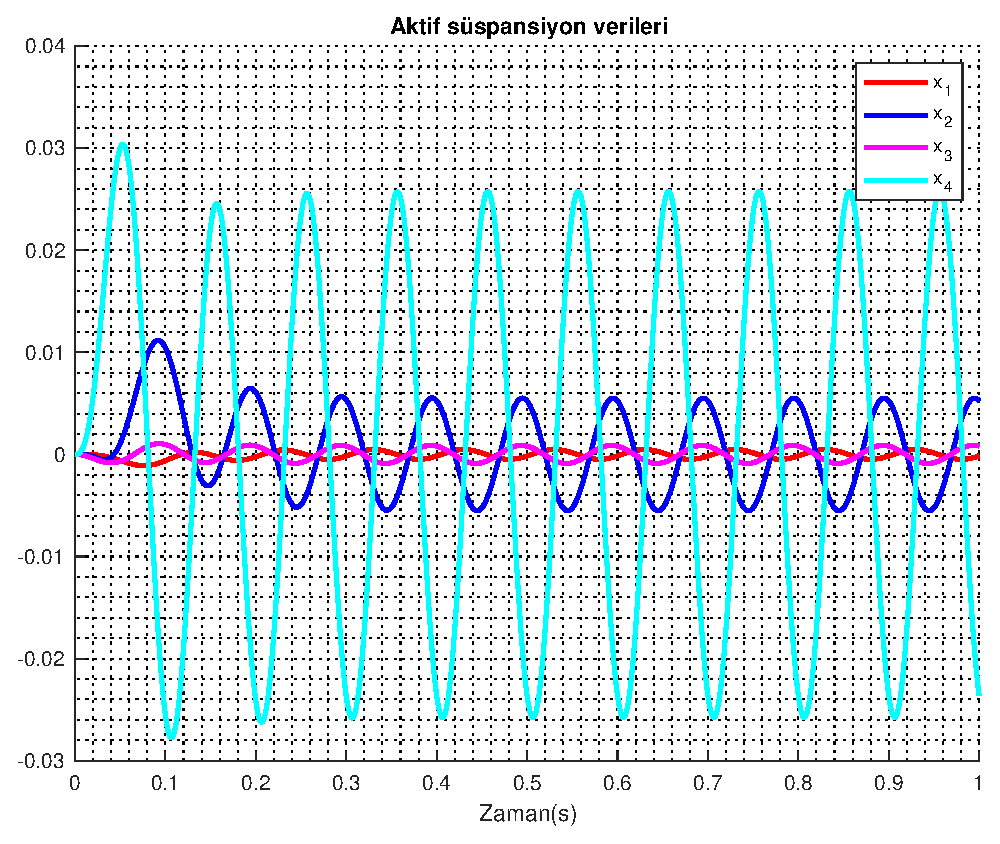
\includegraphics[width=0.75\textwidth]{plot1}
    \caption{Extra soru için elde edilen çizim}
    \label{fig:plot1}
\end{figure}

\begin{figure}[!htb]
    \centering
    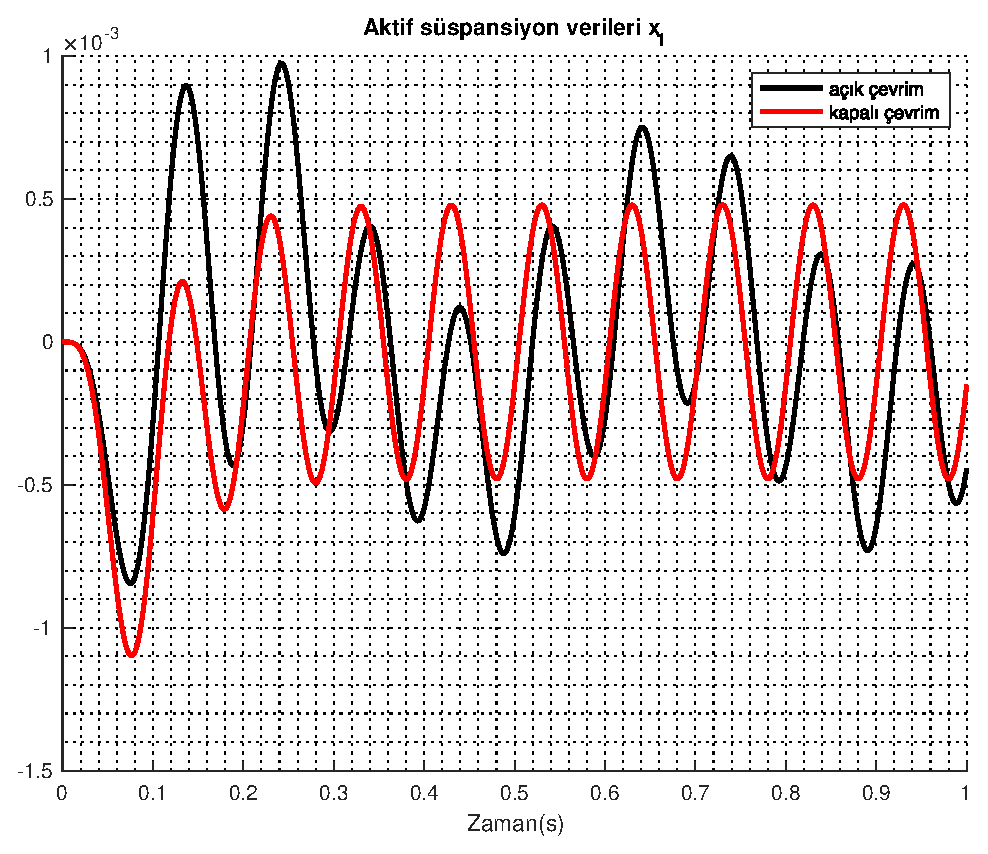
\includegraphics[width=0.75\textwidth]{plot2}
    \caption{Açık ve kapalı çevrim $x_1$ karşılaştırması}
\end{figure}

\begin{figure}[!htb]
    \centering
    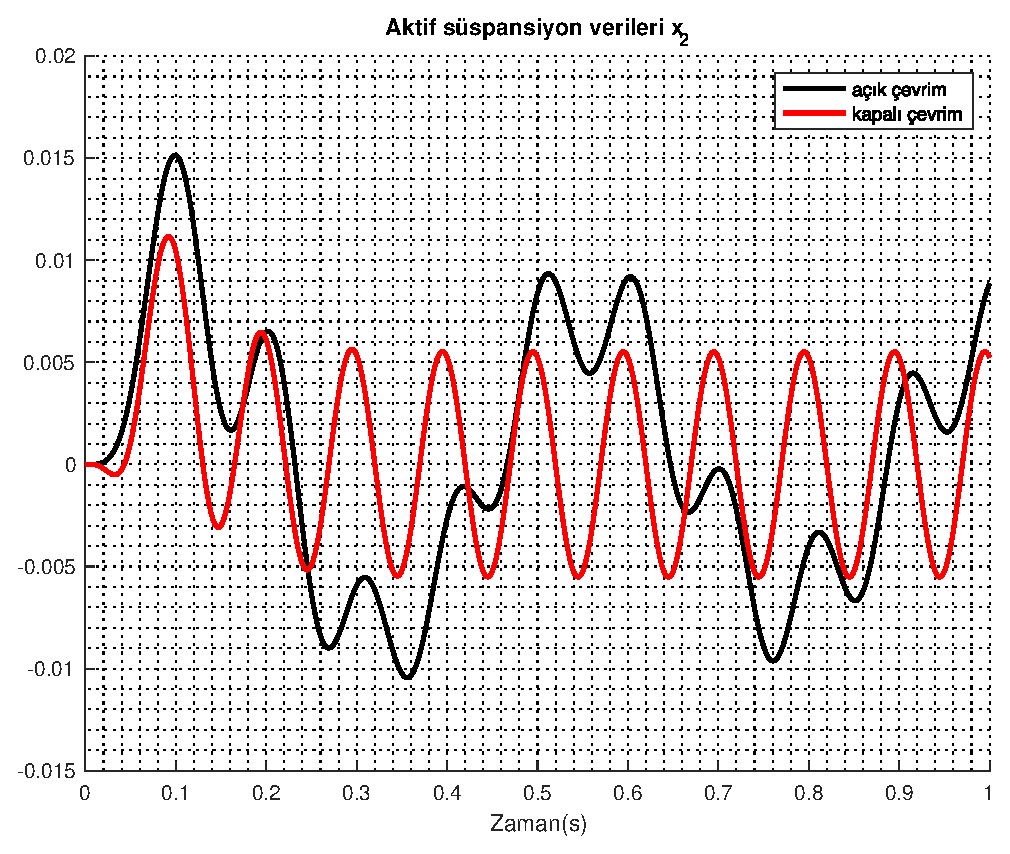
\includegraphics[width=0.75\textwidth]{plot3}
    \caption{Açık ve kapalı çevrim $x_2$ karşılaştırması}
\end{figure}

\begin{figure}[!htb]
    \centering
    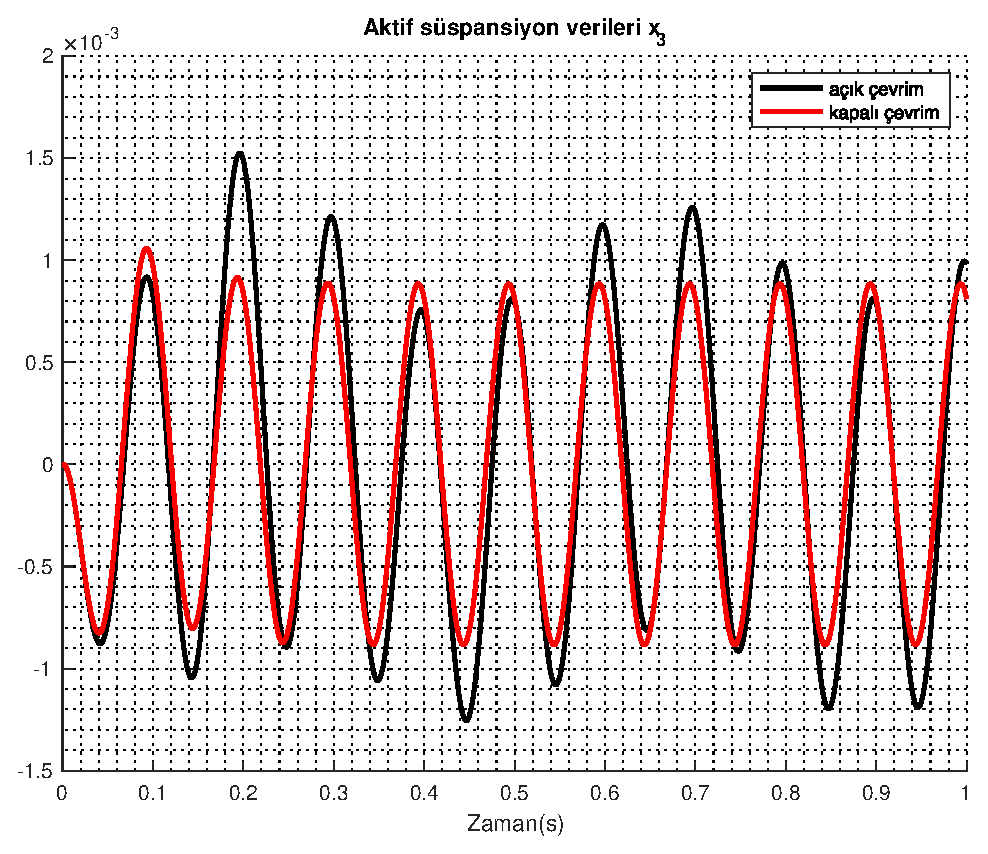
\includegraphics[width=0.75\textwidth]{plot4}
    \caption{Açık ve kapalı çevrim $x_3$ karşılaştırması}
\end{figure}

\begin{figure}[!htb]
    \centering
    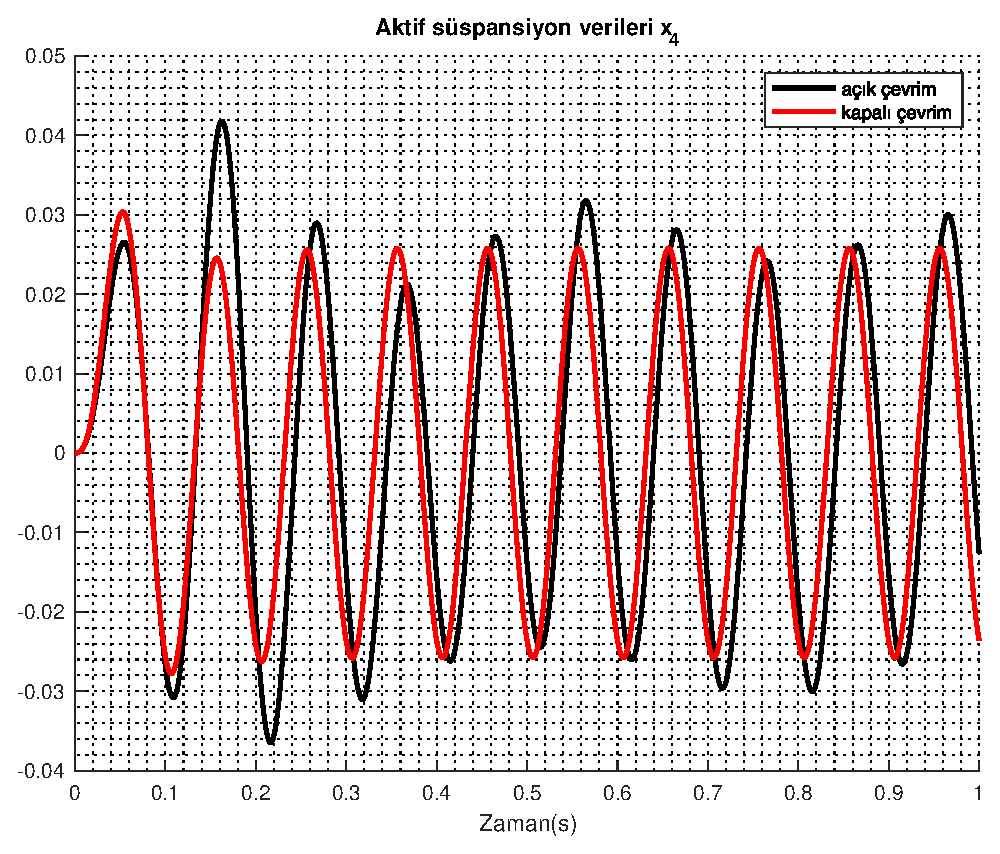
\includegraphics[width=0.75\textwidth]{plot5}
    \caption{Açık ve kapalı çevrim $x_4$ karşılaştırması}
\end{figure}
